\documentclass[12pt]{article}
\usepackage[margin=1in]{geometry}
\usepackage{graphicx}
\graphicspath{ {images/} }
\usepackage{fontspec}
\setmainfont[Path=/usr/share/fonts/truetype/calibri/,
    BoldItalicFont=CALIBRIZ.ttf,
    BoldFont      =CALIBRIB.ttf,
    ItalicFont    =CALIBRII.ttf]{Calibri.ttf}
\title{Lab 05: Work and Energy with an Inclined Plane}
\author{Adris Jautakas, partnered with Matthew Kendall}
\date{January 22, 2018}
\begin{document}
    \maketitle
    \pagebreak
    \section*{Abstract}
        \begin{quote}
        {\textit {\small 
            This experiment observes the laws of Energy and how they can be
            utilized to express changes in a system as a whole. Using a cart
            suspended against a ramp via pulley, we calculated the work done
            by friction on the system as the cart rolls down and concluded that
            energy equations are useful in determining a variety of features
            and properties of a system even under the influence of friction.
        } }
        \end{quote}

    \section{Introduction}
        \par Energy dynamics and the conservation of energy in a system are 
        physical properties that can be used to greatly simplify and explain 
        physical phenomena. Instead of modeling scenarios on a case by case 
        basis on rails with each component of motion and energy transfer 
        calculated, energy dynamics can generalize and describe the change of a
        system across an arbitrary number of events.
        \par Force, energy, and friction can be described using energy dynamics.
        In a system, friction can decrease the energy of a system and can thus
        be considered the change in energy in a system. In this lab, we 
        calculated the work of friction and the frictional force of a cart
        moving down an incline by finding the change in energy of a
        cart-incline system.
    \section{Materials}
        \begin{itemize}
            \item Board
            \item Cart
            \item Pulley with Clamp
            \item Weight sets attachable to string
            \item String attachable to cart
            \item Protractor
            \item Scale (triple beam balance)
            \item Meterstick
        \end{itemize}

    \section{Methods}
        \subsection{Experiment Setup}
            Position the board at an incline to the ground with the pulley
            fixated at its end. Place a cart on the incline and attach it to a
            weight with the string run through the pulley. Measure the angle
            of the incline and the length of the board that the cart traverses.
            Then, increase the mass of the weight by adding extra weights until
            the cart moves down the ramp at a constant velocity when pushed.
            Measure the mass of the weights. Repeat this procedure, but add
            weights until the cart moves up the ramp at a constant velocity
            when pushed.
    \section{Data}
        {\large Experiment A: Cart on a 10 degree incline} \\
        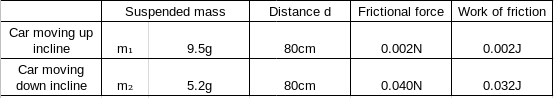
\includegraphics[scale=0.75 ]{Chart10deg.png} \\ \\
        {\large Experiment B: Cart on a 15 degree incline} \\
        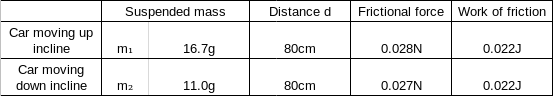
\includegraphics[scale=0.75 ]{Chart15deg.png} \\ \\

    \section{Analysis}
        \subsection{Equations}
            The total energy in this system can be described with this equation:
            \begin{equation}
                E_{net} = W_{PE} - W_G + W_F
            \end{equation}
            where $E_{net}$ is the net energy, $W_{PE}$ is the potential energy,
            $W_G$ is the work done by gravity, and $W_F$ is the energy lost to
            friction. Since $E_{net}$ is constant, as $W_F$ increases, the 
            remaining energy left over decreases and is lost. Since $W = fd$
            for motion, we can express the rest of the terms. For inclined
            surfaces, $F_{\parallel}  = mg\sin{\theta}$ where $\theta$ is the
            angle of the incline. Using our work equation, this leaves us with
            \begin{equation}
                W_G = m_cgd\sin{\theta} + m_wgd
            \end{equation}
            where $d$ is the distance the cart travels, $m_c$ is the mass of
            the cart and $m_w$ is the mass of the weight. Expressing $W_{PE}$ is
            straightforward: $W_{PE} = mgh$. This lets us iscolate for friction
            with the equations
            \begin{equation}
                W_F = E_{net} - W_{PE} + W_G
            \end{equation}
            We can assume the net energy in the system to be 0, because in the
            system the work done by friction and the work done by the weights
            cancel each other out. So we get
            \begin{equation}
                W_F = m_cgd\sin{\theta} + m_wgd - m_cgd
            \end{equation}
            Ideally, this equation would apply to both scenarios of the cart
            moving up the ramp and down the ramp because that only changes
            the sign of $W_F$.

    \section{Conclusion}
        Our results show some consistency between the work of friction done by
        the cart moving up and down, which makes sense considering the normal
        force of the cart on the ramp doesn't change. While some consistency
        was dropped, perhaps due to the inertia of the wheels in the cart or
        on the pulley. We can deduce that the
        principles of energy and its conservation are useful in determining
        physical interactions and transfers of energy without modeling the
        whole system.
\end{document}
